\section{Micro-serviços}

\subsection{Word of caution}
\begin{frame}
Não existe bala de prata!
%\includegraphics[width=\textwidth]{images/nosilver}
\end{frame}



\begin{frame}
Todas estas tecnologias...
\begin{itemize}
	\item Docker
	\item Golang
	\item nodejs
	\item Angular
	\item ...
\end{itemize}
passarão ou encontrarão um nicho, como...
\begin{itemize}
	\item Cobol
	\item Assembly
	\item C
	\item SQL
\end{itemize}
encontraram.

Certamente nenhuma delas será usada para resolver todos os problemas.
\end{frame}


\begin{frame}
\begin{quotation}
	The hype cycle is a branded graphical presentation developed and used by the American research, advisory and information technology firm Gartner, for representing the maturity, adoption and social application of specific technologies.
\end{quotation}

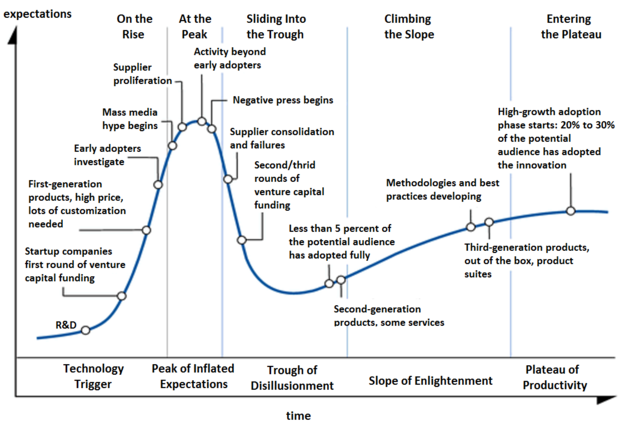
\includegraphics[width=.7\textwidth]{images/gartner-hype-cycle-overview}
\end{frame}

\begin{frame}
\begin{scriptsize}
\begin{enumerate}
\item Technology Trigger -- A potential technology breakthrough kicks things off. Early proof-of-concept stories and media interest trigger significant publicity. Often no usable products exist and commercial viability is unproven.
\item Peak of Inflated -- Expectations	Early publicity produces a number of success stories—often accompanied by scores of failures. Some companies take action; most don't.
\item Trough of Disillusionment	-- Interest wanes as experiments and implementations fail to deliver. Producers of the technology shake out or fail. Investment continues only if the surviving providers improve their products to the satisfaction of early adopters.
\item  Slope of Enlightenment -- More instances of how the technology can benefit the enterprise start to crystallize and become more widely understood. Second- and third-generation products appear from technology providers. More enterprises fund pilots; conservative companies remain cautious.
\item Plateau of Productivity -- Mainstream adoption starts to take off. Criteria for assessing provider viability are more clearly defined. The technology's broad market applicability and relevance are clearly paying off.
\end{enumerate}
\end{scriptsize}
Fonte: Wikipedia
\end{frame}

\begin{frame}
\begin{quotation}
	We tend to overestimate the effect of a technology in the short run and underestimate the effect in the long run.[3][4]
\end{quotation}	
\end{frame}

\begin{frame}
Microsserviços está próximo do pico da desilusão.
\includegraphics[width=1.1\textwidth]{images/gartner-hype-cycle-2017}
\end{frame}


\subsection{Visão Geral}
\begin{frame}
Monolítico x Micro-serviços
\end{frame}

\begin{frame}{Monolito}
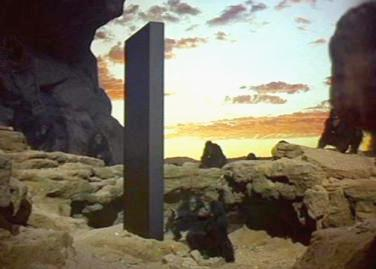
\includegraphics[width=.6\textwidth]{images/monolith_2001}

\href{http://www.imdb.com/title/tt0062622/}{2001 Space Odyssey}
\end{frame}

\begin{frame}{Monolito}
Um bloco com lógica. Por exemplo, um MVC é um sistema monolítico.

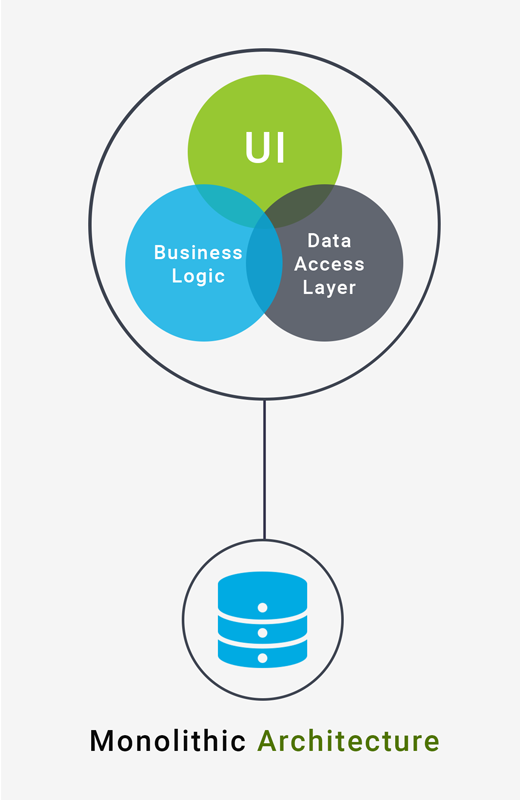
\includegraphics[width=.4\textheight]{images/monolith_arc}

\href{http://nodexperts.com/blog/microservice-vs-monolithic/}{Fonte}
\end{frame}

\begin{frame}{Scala}
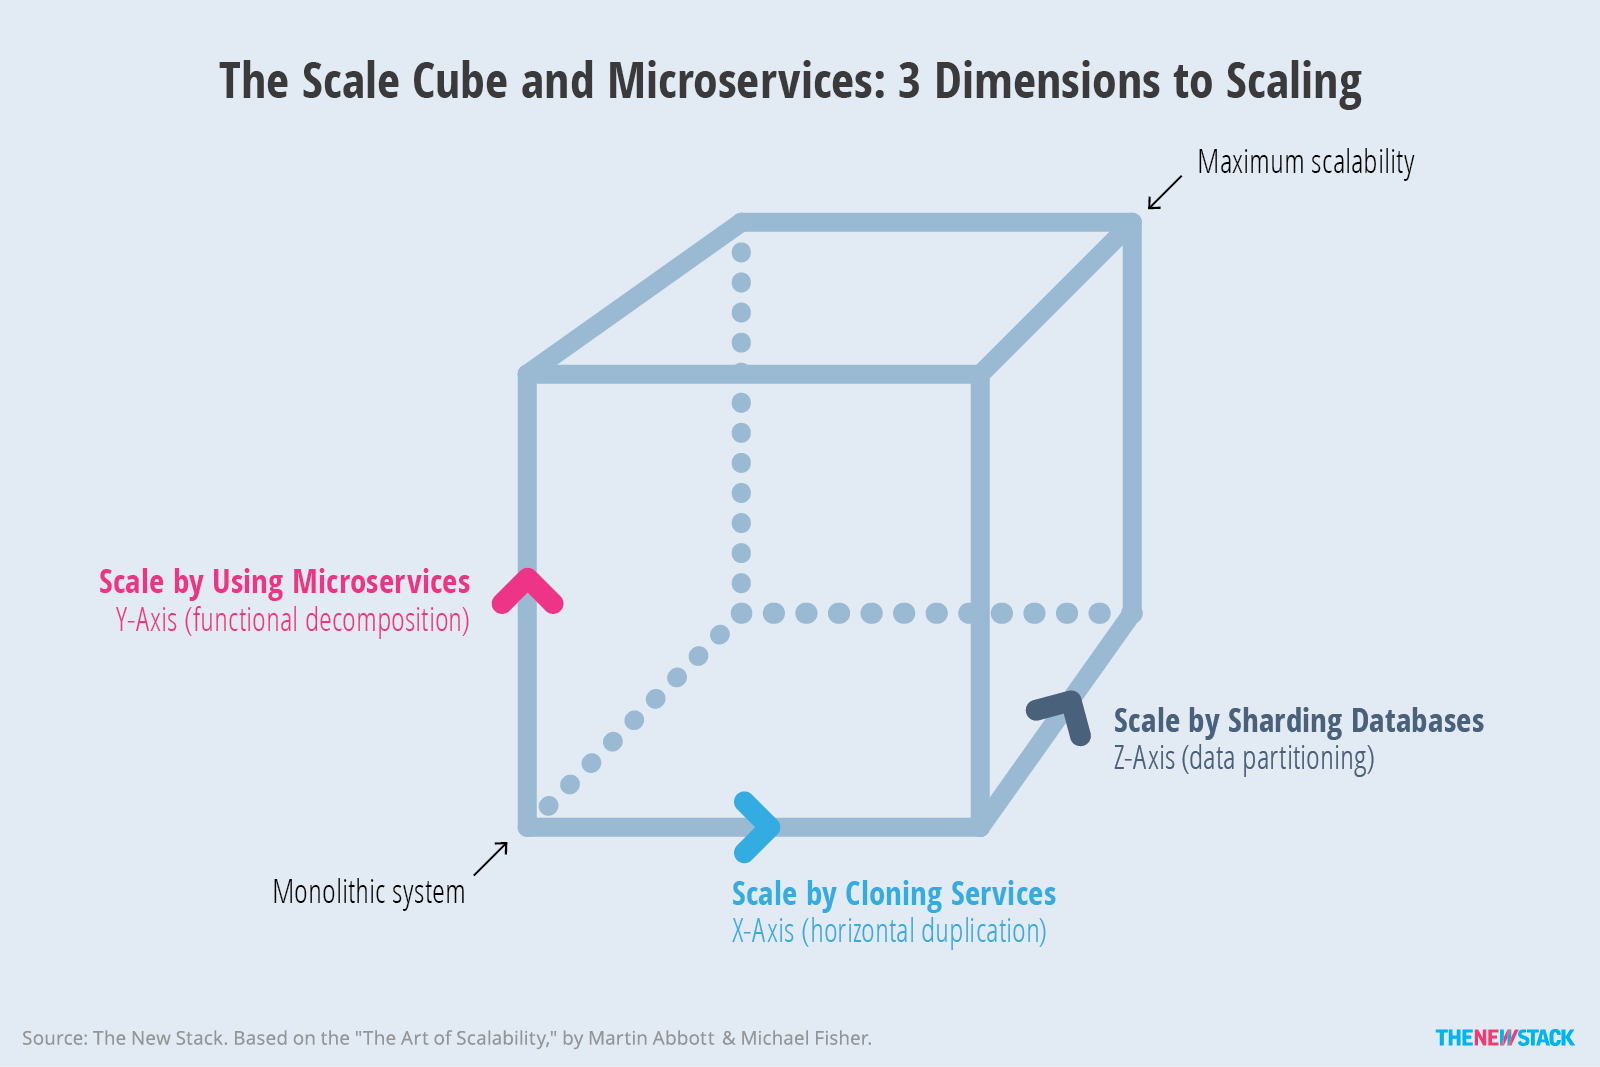
\includegraphics[width=\textheight]{images/microservices_scale}

\href{https://thenewstack.io/from-monolith-to-microservices/}{Fonte}
\end{frame}



\begin{frame}{Micro-serviços}
Blocos especializados

\includegraphics[width=.9\textheight]{images/microservices_arc}

\href{http://nodexperts.com/blog/microservice-vs-monolithic/}{Fonte}
\end{frame}


\subsection{Monolitos}
\begin{frame}{Monolítico}
Exemplos de aplicações monolíticas de sucesso são pervasivos.

\pause Ciclo bem entendido:
\begin{itemize}
	\item Desenvolva
	\item Teste
	\item Implante
	\item Escale
	\item loop
\end{itemize}
\end{frame}

%https://medium.com/@bfil/microservices-are-a-silver-bullet-f745d2b41dca

\begin{frame}{Monolítico}
Com o passar do tempo, tornam-se gigantes que não podem ser movidos ou guiados. A complexidade é grande demais para qualquer indivíduo entender todo o sistema.
\end{frame}

\begin{frame}{Monolítico}
Desenvolvimento ágil se torna impossível. 

Implantações são custosas então são evitadas. Cada nova implantação traz muitas novas mudanças. Risco de problemas é maior. Muito cuidado é necessário. Implantações se tornam mais custosas. loop

Até debugar o sistema é mais complicado. Como carregar tudo no Eclipse? \pause Como atacar o problema?
\end{frame}

\begin{frame}{Monolítico}
Se está funcionando, por quê trocar?

\pause

\begin{itemize}
	\item Mais fácil estender?
	\item Mais fácil de escalar?
	\item Mais fácil de tornar tolerante a falhas?
\end{itemize}
\end{frame}


\subsection{Micro-serviço}

\begin{frame}{Micro-serviços}
``Small autonomous services that work together, modelled around a business domain.''
\end{frame}

\begin{frame}{Micro-serviço}
Ideia semelhante à programação paralela:
\begin{itemize}
	\item Paralelismo de dados: trate dados diferentes em blocos diferentes.
	\item Paralelismo de tarefas: trate funções diferentes em blocos diferentes.
\end{itemize}

\pause\alert{Particionamento}
\end{frame}

Serviço de browsing pode ser replicado mais que de ordering, por exemplo.

\begin{frame}{Particionamento}
\begin{itemize}
	\item Cada componente executa um serviço... bem.
	\item Cada time foca-se em um problema.
\end{itemize}
\end{frame}

\begin{frame}{Escalas diferentes para blocos diferentes}
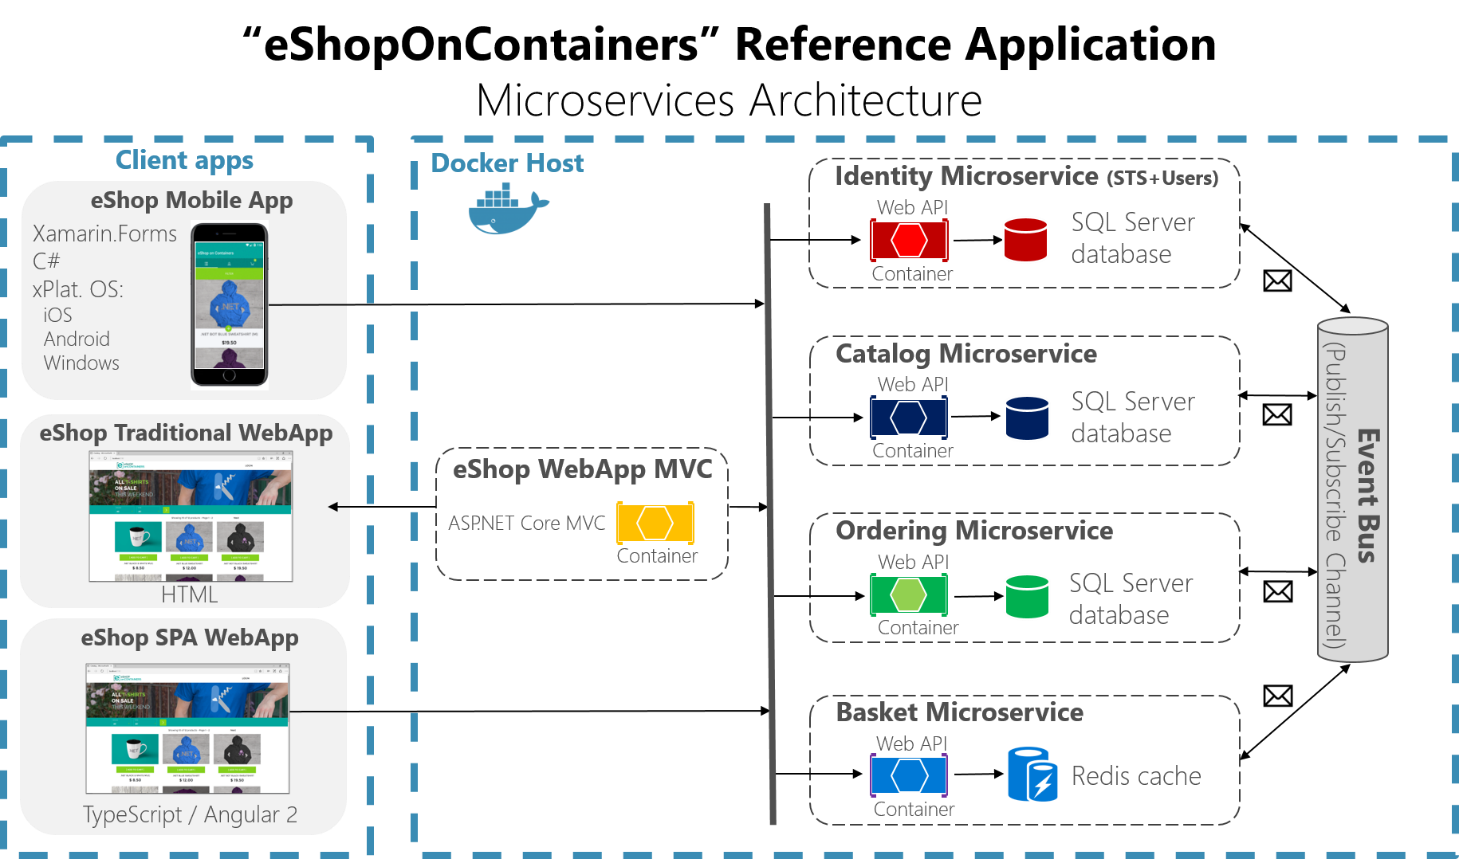
\includegraphics[width=.7\textwidth]{images/microservice_sample}

\href{https://docs.microsoft.com/en-us/dotnet/standard/microservices-architecture/multi-container-microservice-net-applications/microservice-application-design}{Fonte}
\end{frame}

\begin{frame}{Particionamento}
\begin{itemize}
	\item Mudanças são mais contidas (em um simples serviço)
	\item Serviços são desenvolvidos e implantados em paralelo e independentemente
	\item A organização do time de desenvolvimento reflete a organização do sistema
\end{itemize}
\end{frame}

\begin{frame}{Particionamento}
\begin{itemize}
	\item Separe componentes que tem requisitos conflitantes:
	\begin{itemize}
		\item CPU
		\item E/S
		\item Memória
	\end{itemize}
	\item Escale-os independentemente
\end{itemize}
\end{frame}

\begin{frame}{Exemplo: Netflix}
\begin{itemize}
	\item \url{https://youtu.be/57UK46qfBLY}
	\item \url{https://youtu.be/CZ3wIuvmHeM}
\end{itemize}
\end{frame}

\begin{frame}{Exemplos}
\begin{itemize}
	\item ``...over five hundred services... we don't know how many...''
	\item ``...availability of 9.995...'' (< 16 segundos por ano)
	\item ``... four days down... ... moved to the cloud''
	\item ``... it is not if failures will happen... ... it is when it happens...'' 
\end{itemize}

\end{frame}

\begin{frame}{Para aprender mais}
\begin{itemize}
	\item \url{https://youtu.be/wgdBVIX9ifA}
	\item \url{https://youtu.be/PFQnNFe27kU}
	\item \url{https://youtu.be/Ijs55IA8DIk}
	\item \url{https://www.slideshare.net/chris.e.richardson/microservices-pattern-language-microxchg-microxchg2016}
	\item \url{https://martinfowler.com/articles/microservices.html}
	
\end{itemize}
\end{frame}
